% SAT to orthogonal vectors (generated by figs_c3ch10.py).
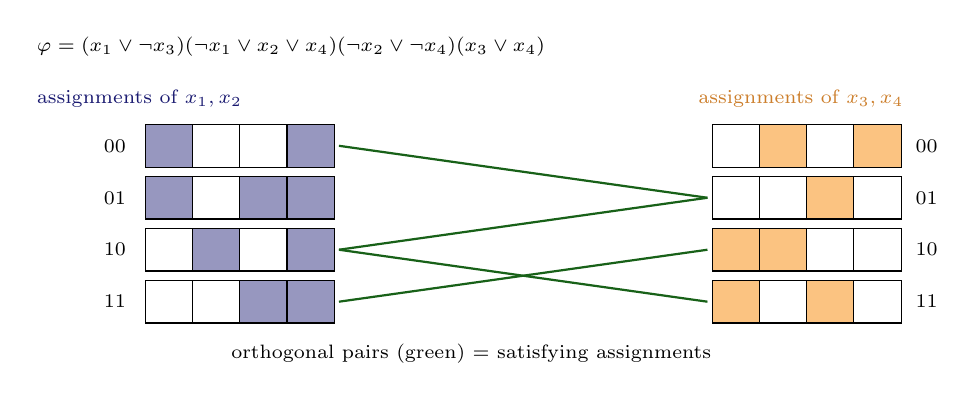
\begin{tikzpicture}[x=6mm,y=6mm,every node/.style={font=\scriptsize}]
\node[anchor=west] at (-0.5,2.1) {$\varphi=(x_1\lor\neg x_3)(\neg x_1\lor x_2\lor x_4)(\neg x_2\lor\neg x_4)(x_3\lor x_4)$};
\node[anchor=west,MidnightBlue] at (-0.5,1.0) {assignments of $x_1,x_2$};
\node[anchor=west,BurntOrange!80!black] at (13.5,1.0) {assignments of $x_3,x_4$};
\node[anchor=east] at (1.8,0.0) {$00$};
\draw[fill=MidnightBlue!45] (2,-0.45) rectangle (3,0.45);
\draw[fill=white] (3,-0.45) rectangle (4,0.45);
\draw[fill=white] (4,-0.45) rectangle (5,0.45);
\draw[fill=MidnightBlue!45] (5,-0.45) rectangle (6,0.45);
\node[anchor=east] at (1.8,-1.1) {$01$};
\draw[fill=MidnightBlue!45] (2,-1.55) rectangle (3,-0.6500000000000001);
\draw[fill=white] (3,-1.55) rectangle (4,-0.6500000000000001);
\draw[fill=MidnightBlue!45] (4,-1.55) rectangle (5,-0.6500000000000001);
\draw[fill=MidnightBlue!45] (5,-1.55) rectangle (6,-0.6500000000000001);
\node[anchor=east] at (1.8,-2.2) {$10$};
\draw[fill=white] (2,-2.6500000000000004) rectangle (3,-1.7500000000000002);
\draw[fill=MidnightBlue!45] (3,-2.6500000000000004) rectangle (4,-1.7500000000000002);
\draw[fill=white] (4,-2.6500000000000004) rectangle (5,-1.7500000000000002);
\draw[fill=MidnightBlue!45] (5,-2.6500000000000004) rectangle (6,-1.7500000000000002);
\node[anchor=east] at (1.8,-3.3000000000000003) {$11$};
\draw[fill=white] (2,-3.7500000000000004) rectangle (3,-2.85);
\draw[fill=white] (3,-3.7500000000000004) rectangle (4,-2.85);
\draw[fill=MidnightBlue!45] (4,-3.7500000000000004) rectangle (5,-2.85);
\draw[fill=MidnightBlue!45] (5,-3.7500000000000004) rectangle (6,-2.85);
\node[anchor=west] at (18.1,0.0) {$00$};
\draw[fill=white] (14,-0.45) rectangle (15,0.45);
\draw[fill=BurntOrange!45] (15,-0.45) rectangle (16,0.45);
\draw[fill=white] (16,-0.45) rectangle (17,0.45);
\draw[fill=BurntOrange!45] (17,-0.45) rectangle (18,0.45);
\node[anchor=west] at (18.1,-1.1) {$01$};
\draw[fill=white] (14,-1.55) rectangle (15,-0.6500000000000001);
\draw[fill=white] (15,-1.55) rectangle (16,-0.6500000000000001);
\draw[fill=BurntOrange!45] (16,-1.55) rectangle (17,-0.6500000000000001);
\draw[fill=white] (17,-1.55) rectangle (18,-0.6500000000000001);
\node[anchor=west] at (18.1,-2.2) {$10$};
\draw[fill=BurntOrange!45] (14,-2.6500000000000004) rectangle (15,-1.7500000000000002);
\draw[fill=BurntOrange!45] (15,-2.6500000000000004) rectangle (16,-1.7500000000000002);
\draw[fill=white] (16,-2.6500000000000004) rectangle (17,-1.7500000000000002);
\draw[fill=white] (17,-2.6500000000000004) rectangle (18,-1.7500000000000002);
\node[anchor=west] at (18.1,-3.3000000000000003) {$11$};
\draw[fill=BurntOrange!45] (14,-3.7500000000000004) rectangle (15,-2.85);
\draw[fill=white] (15,-3.7500000000000004) rectangle (16,-2.85);
\draw[fill=BurntOrange!45] (16,-3.7500000000000004) rectangle (17,-2.85);
\draw[fill=white] (17,-3.7500000000000004) rectangle (18,-2.85);
\draw[ForestGreen!70!black,thick] (6.1,0.0) -- (13.9,-1.1);
\draw[ForestGreen!70!black,thick] (6.1,-2.2) -- (13.9,-1.1);
\draw[ForestGreen!70!black,thick] (6.1,-2.2) -- (13.9,-3.3000000000000003);
\draw[ForestGreen!70!black,thick] (6.1,-3.3000000000000003) -- (13.9,-2.2);
\node[align=center] at (8.9,-4.4) {orthogonal pairs (green) $=$ satisfying assignments};
\end{tikzpicture}
